\definecolor{redpoint}{RGB}{160, 20, 35}
\definecolor{bluepoint}{RGB}{0, 114, 206}
\definecolor{circlecol}{RGB}{125, 125, 130}
\definecolor{linecol}{RGB}{135, 135, 140}
\definecolor{redtext}{RGB}{160, 20, 35}
\definecolor{bluetext}{RGB}{40, 115, 180}

\resizebox{0.7\textwidth}{!}{%
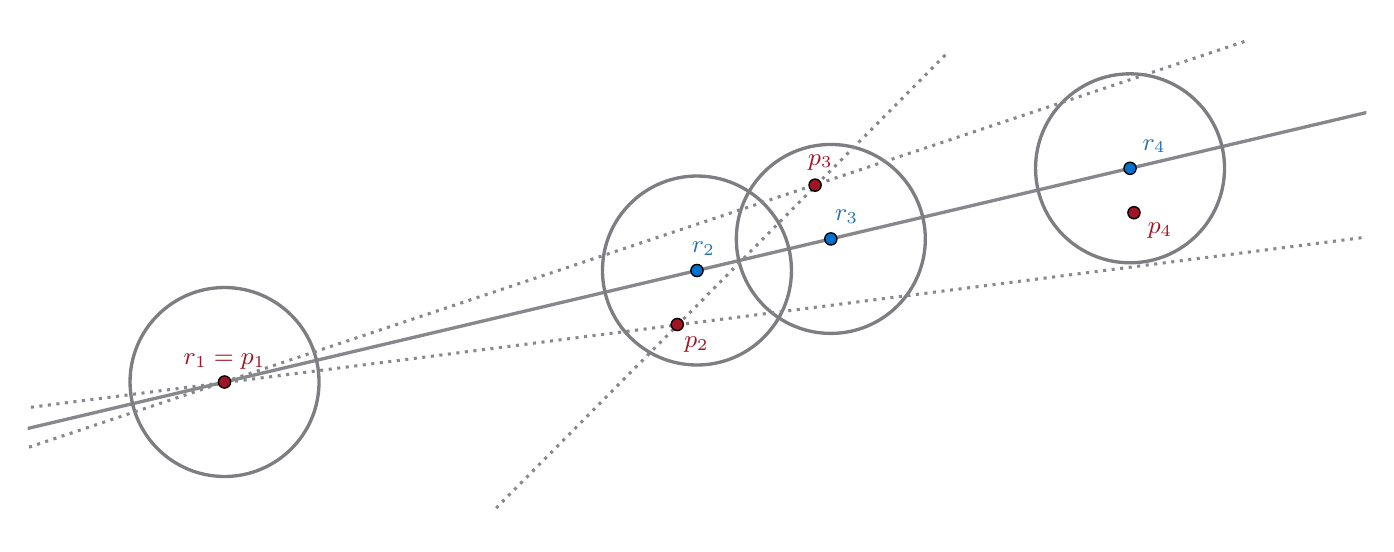
\begin{tikzpicture}[x=1cm, y=1cm]
    \clip (-2.5,-1.8) rectangle (14.5, 4.5);

    % Line coordinates for the main line
    % Passing through r1 at (0,0) with a slope of about 0.236
    % Let r1 = (0,0)
    % Let r2 = (6, 1.416)
    % Let r3 = (7.7, 1.817)
    % Let r4 = (11.5, 2.714)
    
    \coordinate (r1) at (0,0);
    \coordinate (r2) at (6, 1.416);
    \coordinate (r3) at (7.7, 1.817);
    \coordinate (r4) at (11.5, 2.714);

    % Red points
    \coordinate (p1) at (0,0);
    \coordinate (p2) at (5.75, 0.73);
    \coordinate (p3) at (7.5, 2.5);
    \coordinate (p4) at (11.55, 2.15);

    % Main solid line
    \draw[linecol, line width=1.2pt] (-3, -0.708) -- (15, 3.54);

    % Circles
    \draw[circlecol, line width=1.2pt] (r1) circle (1.2);
    \draw[circlecol, line width=1.2pt] (r2) circle (1.2);
    \draw[circlecol, line width=1.2pt] (r3) circle (1.2);
    \draw[circlecol, line width=1.2pt] (r4) circle (1.2);

    % Dotted tangent-like / boundary lines from r1
    % Upper ray from (0,0) through top of middle circles:
    % p1-p3
    \draw[linecol, dotted, line width=1.1pt] (-3, -1) -- (13, 4.34);
    
    % p1p2
    \draw[linecol, dotted, line width=1.1pt] (-3, -0.39) -- (14.5, 1.84);
    
    % Diagonal line passing through p2 and p3:
    \draw[linecol, dotted, line width=1.1pt] (3.45, -1.6) -- (9.2, 4.2);

    % Draw blue points (centers of circles)
    % r1 is overlaid by p1
    \filldraw[fill=bluepoint, draw=black, line width=0.5pt] (r2) circle (2.2pt);
    \filldraw[fill=bluepoint, draw=black, line width=0.5pt] (r3) circle (2.2pt);
    \filldraw[fill=bluepoint, draw=black, line width=0.5pt] (r4) circle (2.2pt);

    % Draw red points
    \filldraw[fill=redpoint, draw=black, line width=0.5pt] (p1) circle (2.2pt);
    \filldraw[fill=redpoint, draw=black, line width=0.5pt] (p2) circle (2.2pt);
    \filldraw[fill=redpoint, draw=black, line width=0.5pt] (p3) circle (2.2pt);
    \filldraw[fill=redpoint, draw=black, line width=0.5pt] (p4) circle (2.2pt);

    % Labels
    \node[redtext, anchor=south, font=\small, yshift=1pt] at (p1) {$r_1 = p_1$};
    
    \node[bluetext, anchor=south east, font=\small, xshift=10pt, yshift=2pt] at (r2) {$r_2$};
    \node[redtext, anchor=north west, font=\small, xshift=-1pt, yshift=-1pt] at (p2) {$p_2$};
    
    \node[bluetext, anchor=south west, font=\small, xshift=-2pt, yshift=2pt] at (r3) {$r_3$};
    \node[redtext, anchor=south west, font=\small, xshift=-6pt, yshift=2pt] at (p3) {$p_3$};
    
    \node[bluetext, anchor=south west, font=\small, xshift=1pt, yshift=2pt] at (r4) {$r_4$};
    \node[redtext, anchor=north west, font=\small, xshift=1.5pt, yshift=-0.1pt] at (p4) {$p_4$};

\end{tikzpicture}
}